\chapter{Representation of a Kapchinsky-Vladimirsky (K-V) phase space distribution by concentric ellipses of macroparticles}

In a four-dimensional phase space $(x,x',y,y')$, the Kapchinsky-Vladimirsky distribution presents a constant density in a three-dimensional subspace.  A four-dimensional Gaussian distribution can be written as an integral over K-V distributions..  We represent this phase space by a series of concentric ellipses on which macroparticles of equal weight are placed.  This adds more macroparticles to the exterior of the distribution, which aids observing nonlinear effects on the beam's transverse phase planes.

\section{Transformation to $(I,\phi)$ coordinates}
The canonical transformation between $(J,\phi)$ and $(x,x')$ coordinates has already been computed:
\Begineq
	\begin{pmatrix} x \\ x' \end{pmatrix}
	= \sqrt{2J} 
	\begin{pmatrix} \sqrt{\beta} & 0 \\ -\frac{\alpha}{\sqrt{\beta}} & -\frac{1}{\sqrt{\beta}} \end{pmatrix}
	\begin{pmatrix} \cos\phi \\ \sin\phi \end{pmatrix}
\Endeq
and a 2D Gaussian distribution is given by
\Begineq
	\rho(J,\phi) = \frac{1}{2\pi\varepsilon} e^{-\frac{J}{\varepsilon}}.
\Endeq
Now consider a 4D phase space $(x,x',y,y')$.  Using this framework, a 4D Gaussian distribution is
\begin{align}
	\rho(J_x,\phi_x,J_y,\phi_y) & = \frac{1}{(2\pi)^2 \varepsilon_x \varepsilon_y}\; exp(-\frac{J_x}{\varepsilon_x})\; exp(-\frac{J_y}{\varepsilon_y}) \\
	                            & = \frac{1}{(2\pi)^2 \varepsilon_x \varepsilon_y}\; exp(-\frac{I_1}{\varepsilon}),
\end{align}
where we have used a new set of orthogonal action coordinates:
\begin{align}
	I_1 & = \left( \frac{J_x}{\varepsilon_x} + \frac{J_y}{\varepsilon_y} \right) \varepsilon  \\
	I_2 & = \left( -\frac{J_x}{\varepsilon_y} + \frac{J_y}{\varepsilon_x} \right) \varepsilon
\end{align}
with $\varepsilon = (\frac{1}{\varepsilon_x^2} + \frac{1}{\varepsilon_y^2})^{-1/2}$.  The reverse transformation is also noted:
\begin{align}
	J_x & = \left( \frac{I_1}{\varepsilon_x} - \frac{I_2}{\varepsilon_y} \right) \varepsilon  \\
	J_y & = \left( \frac{I_1}{\varepsilon_y} + \frac{I_2}{\varepsilon_x} \right) \varepsilon.
\end{align}

\textit{Sidenote}: While this transformation is not canonical, its Jacobian determinant $\left\vert\frac{\partial(I_1,I_2,\phi_x,\phi_y)}{\partial(J_x,J_y,\phi_x,\phi_y)}\right\vert$ is still 1.  A canonical version of this transformation is discussed in section \ref{sec:canon}.

The K-V distribution becomes
\Begineq
	\rho(I_1,I_2,\phi_x,\phi_y) = \frac{1}{A} \delta(I_1 - \xi),
\Endeq
where $A$ is a constant which normalizes the distribution to 1.  By choosing a particular $\xi$ and iterating over the domain of the three remaining coordinates, one can populate a 3D subspace of constant density.

\section{Limits of iteration}
The weight of a macroparticle is determined by the total weight of the region of phase space it represents.  Because the density $\rho$ is only dependent on $I_1$,
\begin{align}
	q & = \int_{0}^{\infty} dI_1 \int_{I_2}^{I_2 + \Delta I_2} dI_2 \int_{\phi_x}^{\phi_x + \Delta \phi_x} d\phi_x \int_{\phi_y}^{\phi_y + \Delta \phi_y} d\phi_y \; \frac{1}{A} \delta(I_1 - \xi) \\
	  & = \frac{1}{A} \Delta I_2 \Delta \phi_x \Delta \phi_y.
\end{align}
To represent the distribution with macroparticles of equal weight, we must partition $(I_2,\phi_x,\phi_y)$-space into regions of equal volume.

The range in $I_2$ to be iterated over is constrained by $J_x$, $J_y \geq 0$.  $J_x, J_y = 0$ give the limits $I_2 \in [-\frac{\varepsilon_x}{\varepsilon_y} I_1, \frac{\varepsilon_y}{\varepsilon_x} I_1]$.  This range is divided into N regions of equal size, with a ring of macroparticles placed in the middle of each region.  The angle variables are also constrained to $\phi_x, \phi_y \in [0, 2\pi]$, with each range divided into $M_x$ and $M_y$ regions, respectively.  Each of these regions will have a particle placed in its center.

Thus, $A = \frac{\varepsilon_x \varepsilon_y}{\varepsilon^2} \xi (2\pi)^2$ and the weight of each macroparticle is
\Begineq
	q = [\frac{\varepsilon_x \varepsilon_y}{\varepsilon^2} \xi (2\pi)^2]^{-1} \frac{\varepsilon_x \varepsilon_y}{\varepsilon^2} \frac{\xi}{N} \frac{2\pi}{M_x} \frac{2\pi}{M_y} = \frac{1}{N M_x M_y}
\Endeq


\subsection*{Sidenote: Canonical version of the transformation}
\label{sec:canon}
To create a canonical transformation, new angle coordinates must also be defined in the same manner as the new action coordinates:
\begin{align}
	\psi_1 & = \left( \frac{\phi_x}{\varepsilon_x} + \frac{\phi_y}{\varepsilon_y} \right) \varepsilon  \\
	\psi_2 & = \left( -\frac{\phi_x}{\varepsilon_y} + \frac{\phi_y}{\varepsilon_x} \right) \varepsilon
\end{align}

Transforming both action and angle coordinates is canonical, because $\mathbf{M}\mathbf{J}\mathbf{M}^T = \mathbf{J}$ for the Jacobian matrix $\mathbf{M} = \frac{\partial(I_1,I_2,\psi_1,\psi_2)}{\partial(J_x,J_y,\phi_x,\phi_y)}$ and $\mathbf{J} = (\begin{smallmatrix} 0 && \mathbf{I} \\ -\mathbf{I} && 0 \end{smallmatrix})$ where $\mathbf{I}$ is the 2x2 identity matrix.

While the limits of iteration for $I_2$ stays the same, the limits for $\psi_1$ and $\psi_2$ are more complicated, since they are constrained by $\phi_1,\phi_2 \in [0,2\pi]$.  The $\lbrace\phi\rbrace \rightarrow \lbrace\psi\rbrace$ transformation rotates the axes, so that the range to iterate over in $\psi_2$ is dependent on the value of $\psi_1$, which is not fixed, and vice versa.  
\begin{figure}[htp]
	\centering
	\begin{tabular}{c c}
	\includegraphics[scale=0.6]{phiblock.eps} & \includegraphics[scale=0.6]{psiblock.eps} \\
	(a) & (b)
	\end{tabular}
	\caption{The region to iterate over in $\lbrace\phi\rbrace$-space (a) is subject to a rotation of axes to $\lbrace\psi\rbrace$-space (b).}
	\label{fig:phipsi}
\end{figure}

However, iterating over this region need not occur along the $\psi_1,\psi_2$ axes, as long as a constant density of points is maintained.  So instead of iterating horizontally over $\psi_1$ and vertically over $\psi_2$, it is possible to iterate diagonally along the axes formed by the edges of the square - but, this is the same as iterating over $\phi_1$ and $\phi_2$, because $\left\vert\frac{\partial(\psi_1,\psi_2)}{\partial(\phi_x,\phi_y)}\right\vert = 1$.

Therefore, the weight of each macroparticle is as before:
\Begineq
	q = \frac{1}{A} \Delta I_2 \Delta \phi_x \Delta \phi_y.
\Endeq


